\chapter{Eksperymenty dla schematu licencyjnego Duolingo Super}
\label{chap:experiments}
\section{Środowisko i metodologia}

Eksperymenty wykonano na komputerze z procesorem Intel Core i5-14600KF (12 rdzeni udostępnionych w WSL2, 3.49~GHz) oraz 16~GB pamięci RAM. System operacyjny: Ubuntu~24.04~LTS uruchomiony w środowisku WSL2. Algorytmy zaimplementowano w Pythonie~3.13 z wykorzystaniem bibliotek NumPy, NetworkX oraz PuLP jako interfejsu do solvera ILP. Każdy pomiar obejmował wyłącznie czas obliczeń; nie uwzględniano czasu generowania instancji ani operacji I/O.

Środowisko badawcze zrealizowano jako zestaw skryptów w języku Python. Oddzielne moduły obsługują benchmark statyczny, symulacje dynamiczne oraz scenariusze rozszerzeń; polecenia CLI umożliwiają uruchamianie pojedynczych algorytmów w trybie diagnostycznym. Przyjęty podział umożliwia równoległe prowadzenie serii eksperymentów oraz sprawną weryfikację jakości metod.

Analizą objęto dwa zbiory danych: (i) syntetyczne grafy losowe, bezskalowe i małoświatowe o 50-450 wierzchołkach, (ii) grafy ego z serwisu Facebook o 53-1035 wierzchołkach. Dla każdej instancji uruchamiano wszystkie algorytmy z limitem 60~s; przekroczenie limitu skutkowało wyłączeniem instancji z dalszych obliczeń. W grafach syntetycznych łącznie odnotowano 10 przekroczeń limitu czasu (algorytm mrówkowy oraz ILP). W grafach rzeczywistych: 8 (mrówkowy), 18 (ILP) i 6 (przeszukiwanie tabu). Pozostałe uruchomienia zakończyły się powodzeniem.

Dla każdego rozmiaru grafów syntetycznych wygenerowano trzy niezależne instancje i wykonano po dwa uruchomienia każdego algorytmu. Analiza grafów ego Facebooka obejmowała po jednym grafie na rozmiar oraz dwa powtórzenia dla każdej pary (graf, algorytm), co umożliwiło oszacowanie zmienności wyników przy zachowaniu budżetu obliczeniowego. W każdej próbie zapisano całkowity koszt licencji, czas wykonania oraz średni koszt licencji na węzeł. Wyniki agregowano jako średnie arytmetyczne. Istotność różnic oceniono testem Friedmana (statystyka $\chi^2_F$, poziom istotności $p$) oraz porównaniami post-hoc metodą Nemenyi’ego. Na benchmarku syntetycznym: $\chi^2_F=577.93$ dla czasu oraz $\chi^2_F=518.01$ dla kosztu licencji na węzeł (w obu przypadkach $p<10^{-100}$), co uzasadnia porównania post-hoc.

Aby ułatwić porównania, ceny licencji znormalizowano. Cenę licencji indywidualnej ustalono na 1, a ceny licencji grupowych przeskalowano zgodnie z pierwotnymi relacjami cenowymi. Dzięki temu możliwe było bardziej przejrzyste porównanie kosztów między różnymi strategiami licencjonowania, niezależnie od ich bezwzględnych wartości.

\section{Duolingo Super na grafach syntetycznych}

\subsection{Statystyki zbiorcze}
Tabela~\ref{tab:duo-synth-summary} zestawia średnie wartości kosztu licencji na wierzchołek oraz czasu dla schematu licencyjnego Duolingo Super. Aby zapewnić porównywalność wyników, analizy statystyczne i wizualizacje oparto na podzbiorze instancji, dla których wszystkie algorytmy zakończyły działanie przed upływem limitu czasu; w praktyce oznacza to przycięcie rozmiarów grafów do zakresu wspólnego dla solvera ILP i algorytmu mrówkowego, które najczęściej przekraczały limit. Solver ILP pozostaje najlepszym punktem odniesienia jakościowego (średni koszt licencji na węzeł 0.445), lecz ma zastosowanie jedynie dla mniejszych instancji. Liczba przekroczeń limitu czasu jest taka sama jak w algorytmie mrówkowym. Wśród metaheurystyk najniższy koszt licencji na węzeł osiąga właśnie algorytm mrówkowy (0.506), natomiast przeszukiwanie tabu zapewnia najlepszy kompromis kosztu licencji na węzeł i czasu w grupie metod przybliżonych. Algorytm zachłanny i algorytm losowy charakteryzują się czasem działania rzędu milisekund, ale tylko pierwszy z nich utrzymuje akceptowalny koszt licencji na węzeł (0.548), podczas gdy algorytm losowy generuje rozwiązania o istotnie wyższym koszcie na węzeł.

\begin{table}[H]
  \centering
  \caption{Średnie wartości kosztu licencji na węzeł i czasu dla schematu licencyjnego Duolingo Super na grafach syntetycznych.}
  \label{tab:duo-synth-summary}
  \begin{tabular}{lrrr}
    \toprule
    \textbf{Algorytm}     & \textbf{Średni koszt/węzeł} & \textbf{Średni koszt} & \textbf{Średni czas [s]} \\
    \midrule
    Algorytm ILP          & 0.445                       & 73.83                 & 2.492                    \\
    Algorytm mrówkowy     & 0.506                       & 83.58                 & 5.124                    \\
    Przeszukiwanie tabu   & 0.500                       & 117.80                & 3.298                    \\
    Algorytm genetyczny   & 0.515                       & 118.36                & 1.222                    \\
    Wyżarzanie symulowane & 0.531                       & 120.90                & 0.975                    \\
    Zbiór dominujący      & 0.542                       & 119.97                & 0.017                    \\
    Algorytm zachłanny    & 0.548                       & 121.94                & 0.001                    \\
    Algorytm losowy       & 0.799                       & 179.90                & 0.001                    \\
    \bottomrule
  \end{tabular}
\end{table}


\subsection{Porównanie algorytmów na grafach syntetycznych}

Rysunki~\ref{fig:duo-synth-cost-random}--\ref{fig:duo-synth-cost-small-world} pokazują wyniki porównywalne z ILP dla grafów losowych i małoświatowych, natomiast dla grafów bezskalowych obserwuje się wyższe koszty.


\begin{figure}[H]
  \centering
  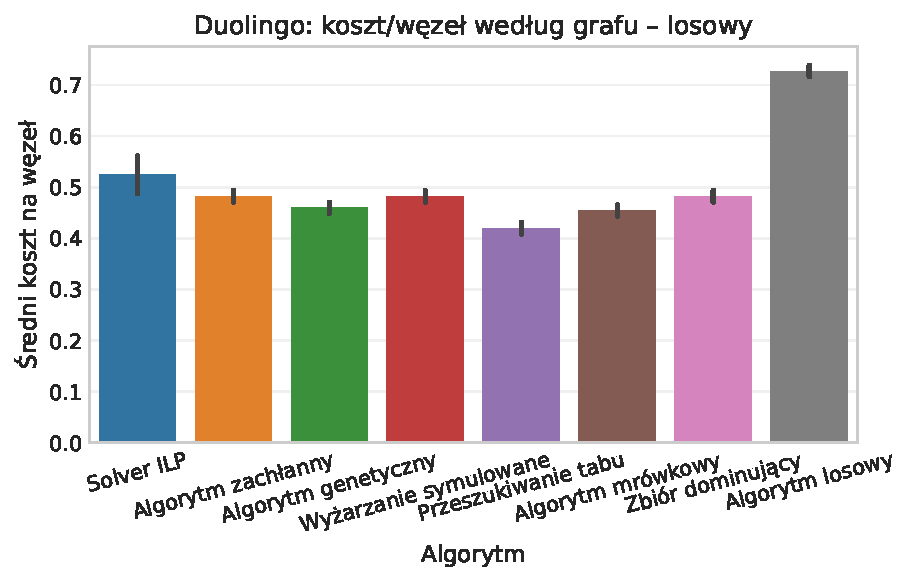
\includegraphics[width=0.65\linewidth]{assets/figures/benchmark/synthetic/duolingo_cost_per_node_by_graph_random.pdf}
  \caption{Koszt licencji na węzeł w zależności od struktury grafu losowego.}
  \label{fig:duo-synth-cost-random}
\end{figure}

\begin{figure}[H]
  \centering
  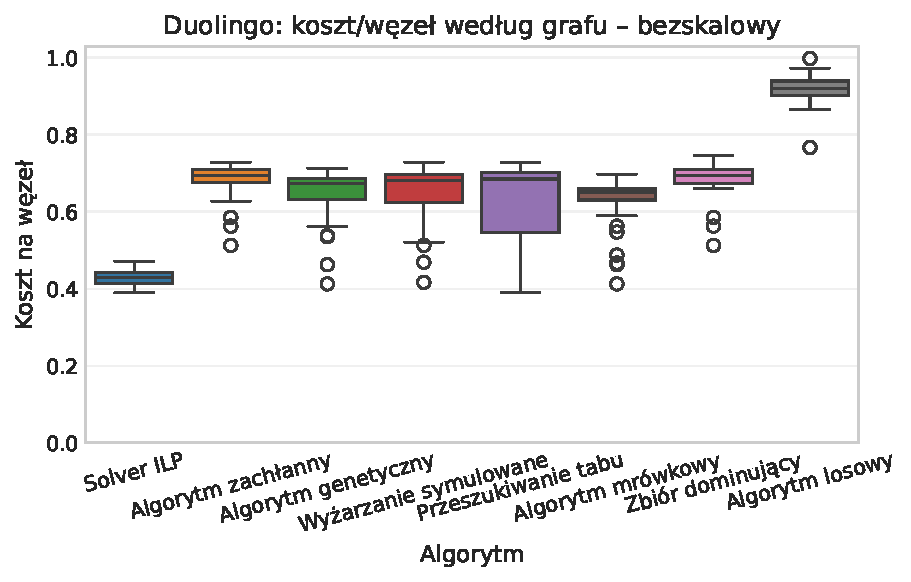
\includegraphics[width=0.65\linewidth]{assets/figures/benchmark/synthetic/duolingo_cost_per_node_by_graph_scale_free.pdf}
  \caption{Koszt licencji na węzeł w zależności od struktury grafu bezskalowego.}
  \label{fig:duo-synth-cost-scale-free}
\end{figure}

\begin{figure}[H]
  \centering
  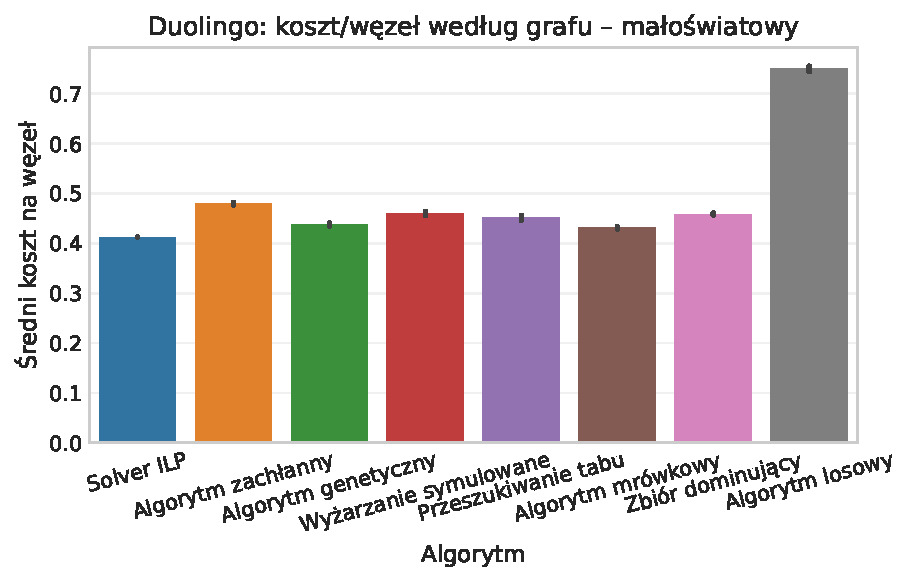
\includegraphics[width=0.65\linewidth]{assets/figures/benchmark/synthetic/duolingo_cost_per_node_by_graph_small_world.pdf}
  \caption{Koszt licencji na węzeł w zależności od struktury grafu małoświatowego.}
  \label{fig:duo-synth-cost-small-world}
\end{figure}

Podobne obserwacje dotyczą czasów wykonania, jak ilustrują rysunki~\ref{fig:duo-synth-time-random}--\ref{fig:duo-synth-time-small-world}. Czasy działania są zbliżone między typami grafów; wyjątkiem są: ILP (średnio krótszy czas na grafach bezskalowych) oraz przeszukiwanie tabu (dłuższy czas na grafach bezskalowych). Pozostałe algorytmy wykazują porównywalne czasy niezależnie od struktury grafu. Tabela~\ref{tab:duo-synth-summary-times} podsumowuje średnie czasów i kosztów licencji na węzeł dla różnych typów grafów.

\begin{figure}[H]
  \centering
  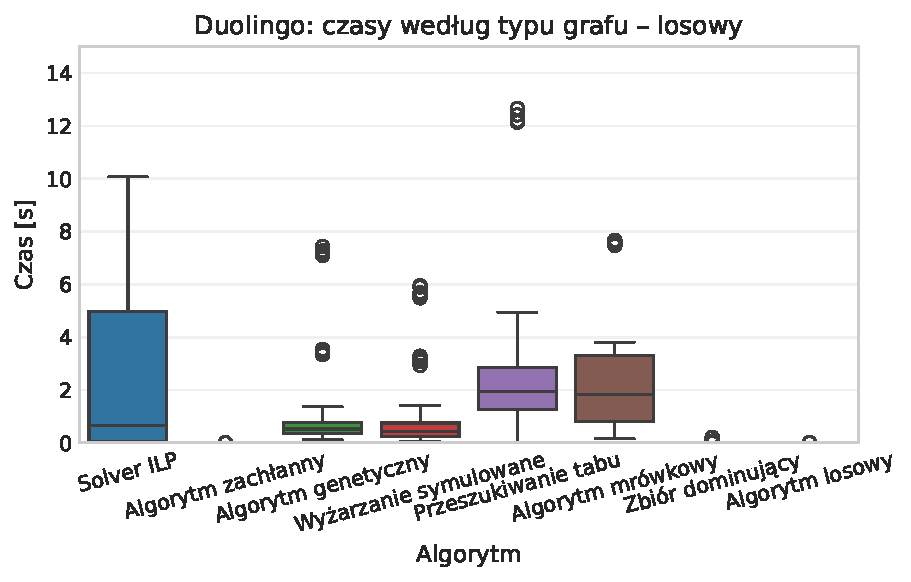
\includegraphics[width=0.65\linewidth]{assets/figures/benchmark/synthetic/duolingo_time_by_graph_random.pdf}
  \caption{Czas wykonania w zależności od struktury grafu losowego.}
  \label{fig:duo-synth-time-random}
\end{figure}

\begin{figure}[H]
  \centering
  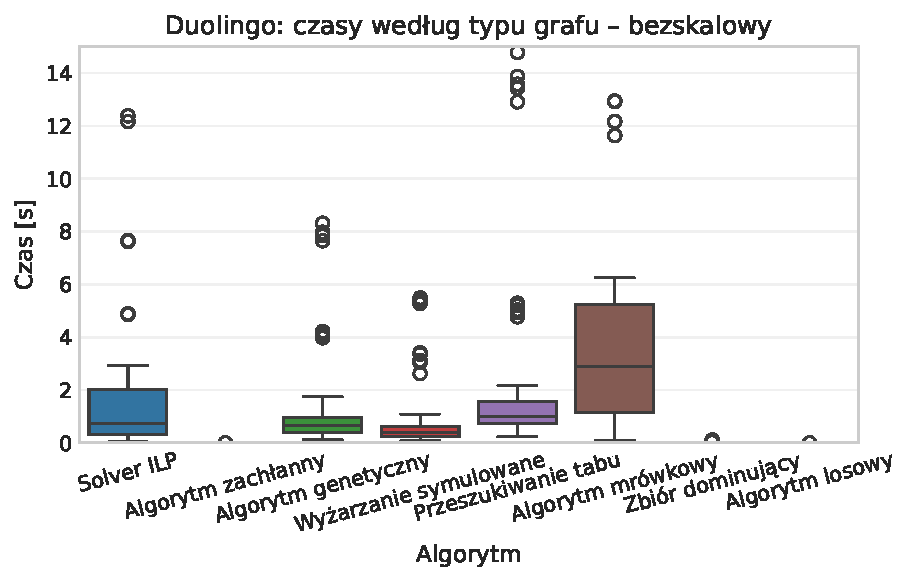
\includegraphics[width=0.65\linewidth]{assets/figures/benchmark/synthetic/duolingo_time_by_graph_scale_free.pdf}
  \caption{Czas wykonania w zależności od struktury grafu bezskalowego.}
  \label{fig:duo-synth-time-scale-free}
\end{figure}

\begin{figure}[H]
  \centering
  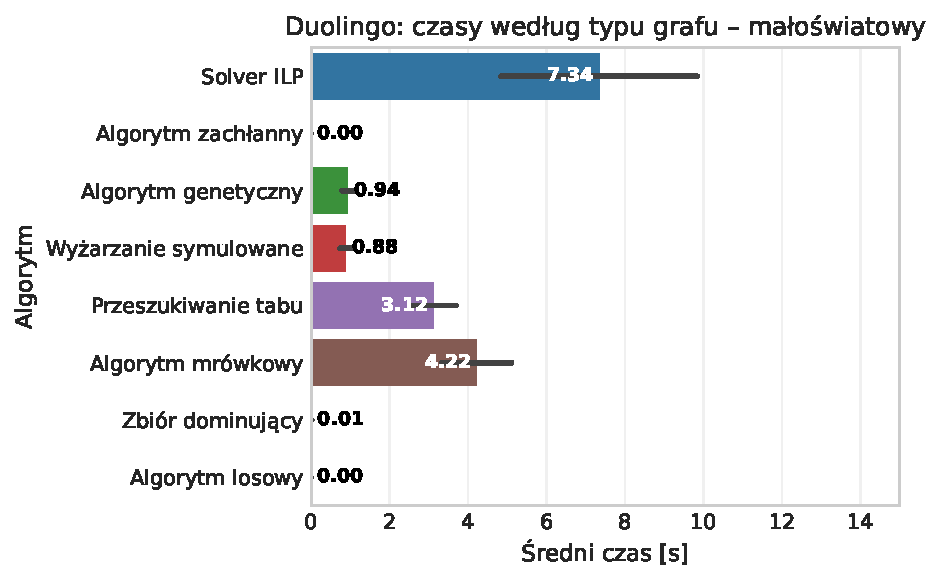
\includegraphics[width=0.65\linewidth]{assets/figures/benchmark/synthetic/duolingo_time_by_graph_small_world.pdf}
  \caption{Czas wykonania w zależności od struktury grafu małoświatowego.}
  \label{fig:duo-synth-time-small-world}
\end{figure}

\begin{table}[H]
  \centering
  \caption{Średnie koszty i czasy na węzeł dla różnych typów grafów (schematy licencyjne Duolingo Super i dominowania rzymskiego).}
  \label{tab:duo-synth-summary-times}
  \begin{tabular}{lcccc}
    \toprule
    \textbf{Licencja}    & \textbf{Typ grafu} & \textbf{Śr. koszt/węzeł} & \textbf{Śr. czas [s]} \\
    \midrule
    Duolingo Super       & Bezskalowy         & 0.661                    & 1.655                 \\
    Duolingo Super       & Losowy             & 0.502                    & 1.598                 \\
    Duolingo Super       & Małoświatowy       & 0.495                    & 1.346                 \\
    dominowanie rzymskie & Bezskalowy         & 0.490                    & 0.913                 \\
    dominowanie rzymskie & Losowy             & 0.344                    & 0.815                 \\
    dominowanie rzymskie & Małoświatowy       & 0.409                    & 1.544                 \\
    \bottomrule
  \end{tabular}
\end{table}



\section{Duolingo Super na grafach rzeczywistych}
W analizie grafów ego z serwisu Facebook pominięto obserwacje, w których algorytm ILP nie zakończył pracy przed limitem czasu (18 przypadków). Dodatkowo odnotowano 8 przekroczeń limitu czasu algorytmu mrówkowego i 6 przypadków w przeszukiwaniu tabu; pozostałe uruchomienia zakończyły się sukcesem.

\begin{table}[H]
  \centering
  \caption{Statystyki kosztu i czasu dla schematu licencyjnego Duolingo Super na grafach rzeczywistych.}
  \label{tab:duo-real-alg}
  \begin{tabular}{lrrr}
    \toprule
    \textbf{Algorytm}     & \textbf{Średni koszt} & \textbf{Śr. koszt/węzeł} & \textbf{Śr. czas [s]} \\
    \midrule
    Algorytm mrówkowy     & 83.58                 & 0.506                    & 5.124                 \\
    Zbiór dominujący      & 119.97                & 0.542                    & 0.017                 \\
    Algorytm genetyczny   & 118.36                & 0.515                    & 1.222                 \\
    Algorytm zachłanny    & 121.94                & 0.548                    & 0.001                 \\
    Algorytm losowy       & 179.90                & 0.799                    & 0.001                 \\
    Wyżarzanie symulowane & 120.90                & 0.531                    & 0.975                 \\
    Przeszukiwanie tabu   & 117.80                & 0.500                    & 3.298                 \\
    \bottomrule
  \end{tabular}
\end{table}
Tabela~\ref{tab:duo-real-alg} wskazuje, że zarówno przeszukiwanie tabu, jak i algorytm mrówkowy zachowują przewagę kosztową nad heurystykami losowymi i zachłannymi, kosztem dłuższego czasu działania.

\subsection{Skalowanie i jakość}

Rysunek~\ref{fig:duo-real-size} ilustruje, że koszt licencji na węzeł pozostaje względnie stabilny niezależnie od liczby wierzchołków, z niewielkimi wahaniami spowodowanymi różnicami między poszczególnymi instancjami grafów. Przeszukiwanie tabu utrzymuje najniższe wartości, a algorytm mrówkowy osiąga wartości zbliżone. Czasy działania rosną łagodnie wraz z rozmiarem grafu i dla największych instancji nie przekraczają kilkudziesięciu sekund; algorytm zachłanny działa rzędu milisekund i jest efektywną procedurą inicjalizacji metaheurystyk. Dodatkowo tabela~\ref{tab:duo-real-size-table} agreguje średnie wartości (przeszukiwanie tabu) dla kolejnych rozmiarów sieci ego i pokazuje, że koszt licencji na węzeł oscyluje w przedziale 0.37--0.56 przy czasie rosnącym od około 2~s do około 33~s dla największych grafów.

\begin{figure}[H]
  \centering
  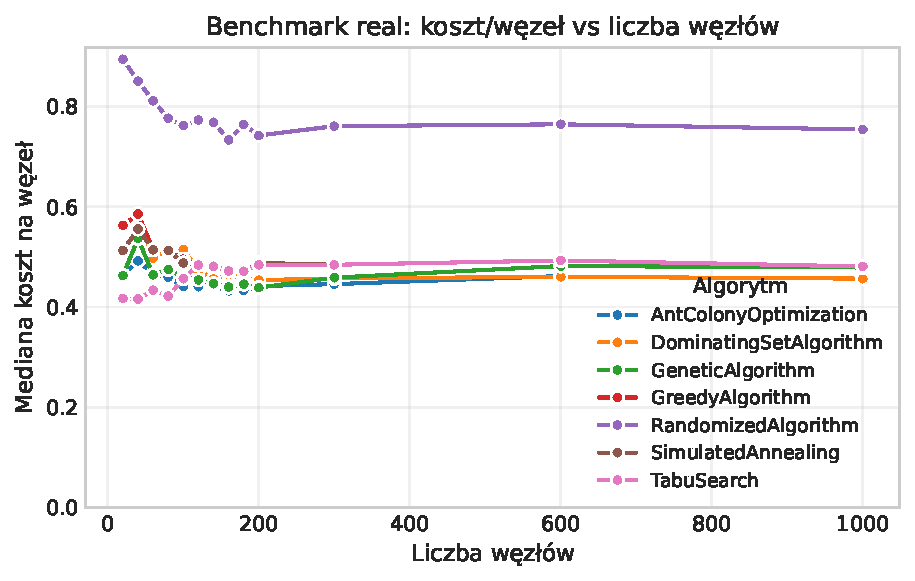
\includegraphics[width=0.48\linewidth]{assets/figures/benchmark/real/cost_per_node_vs_nodes.pdf}
  \hfill
  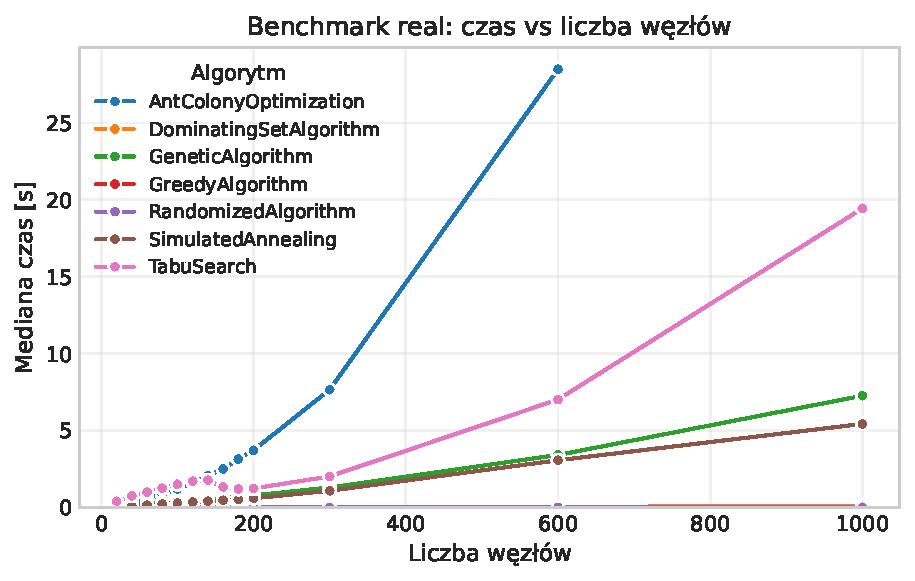
\includegraphics[width=0.48\linewidth]{assets/figures/benchmark/real/time_vs_nodes.pdf}
  \caption{Koszt licencji na węzeł i czas wykonania algorytmów dla schematu licencyjnego Duolingo Super w zależności od liczby wierzchołków (grafy ego Facebook).}
  \label{fig:duo-real-size}
\end{figure}

\begin{table}[H]
  \centering
  \caption{Średni koszt licencji na węzeł i czas (przeszukiwanie tabu) względem liczby wierzchołków w sieciach ego Facebook.}
  \label{tab:duo-real-size-table}
  \begin{tabular}{lrr}
    \toprule
    \textbf{Liczba wierzchołków} & \textbf{Śr. koszt/węzeł} & \textbf{Śr. czas [s]} \\
    \midrule
    53                           & 0.441                    & 2.16                  \\
    62                           & 0.370                    & 3.14                  \\
    151                          & 0.379                    & 6.83                  \\
    169                          & 0.393                    & 8.73                  \\
    225                          & 0.408                    & 12.32                 \\
    334                          & 0.561                    & 32.71                 \\
    \bottomrule
  \end{tabular}
\end{table}


\section{Porównanie z dominowaniem rzymskim}

Porównania schematu licencyjnego Duolingo Super z konfiguracją imitującą dominowanie rzymskie ograniczono do wspólnych instancji grafów i algorytmów. Rysunki~\ref{fig:duo-roman-cost}--\ref{fig:duo-roman-license} zestawiają różnice w kosztach, czasach i strukturze licencji, a tabela~\ref{tab:duo-roman-graph} gromadzi średnie według typu grafu syntetycznego.

\begin{table}[H]
  \centering
  \caption{Średnie czasu i kosztu licencji na węzeł według typu grafu (wspólne instancje).}
  \label{tab:duo-roman-graph}
  \begin{tabular}{lcccc}
    \toprule
    \multirow{2}{*}{\textbf{Typ grafu}} & \multicolumn{2}{c}{\textbf{Duolingo Super}} & \multicolumn{2}{c}{\textbf{dominowanie rzymskie}}                                            \\
                                        & \textbf{Czas [s]}                           & \textbf{Koszt/węzeł}                              & \textbf{Czas [s]} & \textbf{Koszt/węzeł} \\
    \midrule
    Losowy                              & 1.598                                       & 0.502                                             & 0.815             & 0.344                \\
    Bezskalowy                          & 1.655                                       & 0.661                                             & 0.913             & 0.490                \\
    Małoświatowy                        & 1.346                                       & 0.495                                             & 1.544             & 0.409                \\
    \bottomrule
  \end{tabular}
\end{table}

Schemat dominowania rzymskiego osiąga niższy koszt licencji na węzeł we wszystkich typach grafów syntetycznych. Największą przewagę odnotowano w grafach losowych (≈0.158; ≈32\%), następnie w bezskalowych (≈0.171), a najmniejszą w małoświatowych (≈0.086). Czasy działania pozostają porównywalne pomiędzy schematami: w grafach małoświatowych algorytmy dla Duolingo Super działają nieco szybciej, natomiast w losowych i bezskalowych przewagę uzyskuje konfiguracja dominowania rzymskiego. Rysunek~\ref{fig:duo-roman-cost} ilustruje te obserwacje dla pełnego rozkładu kosztów, a rysunek~\ref{fig:duo-roman-time} prezentuje analogiczne dane dotyczące czasów wykonania. Warto zauważyć, że wyższe koszty licencji na węzeł w przypadku Duolingo Super wynikają z ograniczeń w opłacalności licencji grupowych. Licencja grupowa jest ≈2.1-krotnie droższa od indywidualnej, co uzasadnia jej tworzenie dopiero dla grup co najmniej trzech wierzchołków (posiadacz oraz dwaj sąsiedzi). W konsekwencji liczba licencji indywidualnych w schemacie Duolingo Super jest większa, co przekłada się na wyższy średni koszt licencji na węzeł w porównaniu z konfiguracją dominowania rzymskiego.

\begin{figure}[H]
  \centering
  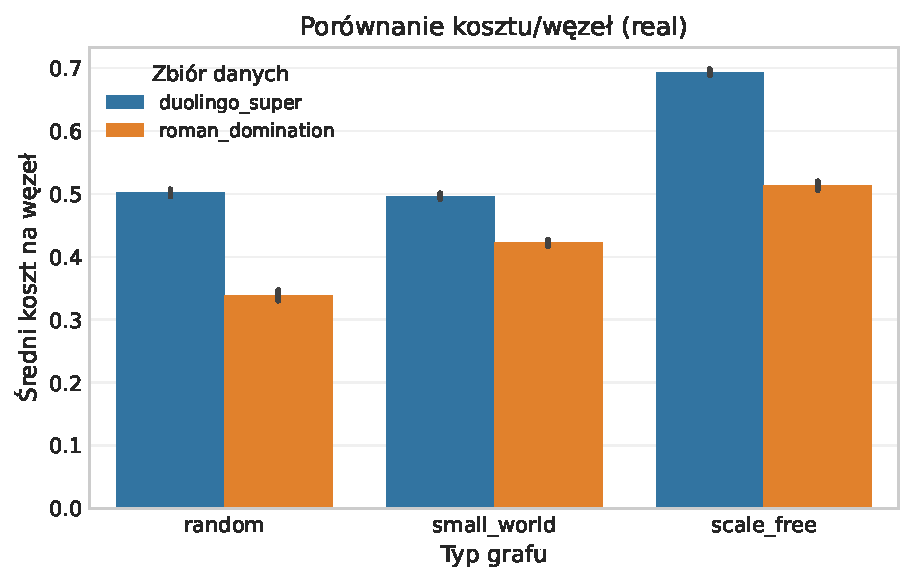
\includegraphics[width=0.6\linewidth]{assets/figures/benchmark/real/duo_vs_roman_cost_per_node_by_graph.pdf}
  \caption{Koszt licencji na węzeł według typu grafu: porównanie konfiguracji licencyjnych Duolingo Super i dominowania rzymskiego.}
  \label{fig:duo-roman-cost}
\end{figure}

\begin{figure}[H]
  \centering
  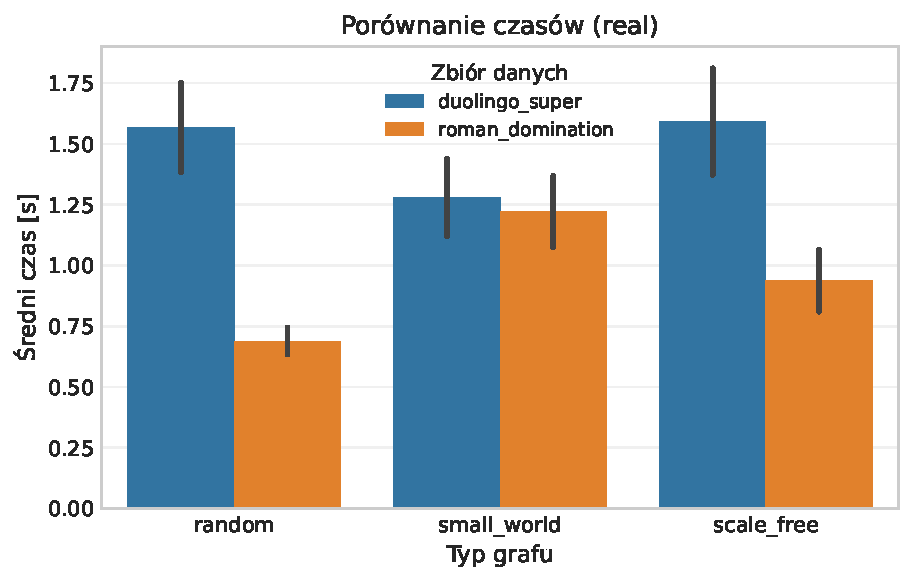
\includegraphics[width=0.6\linewidth]{assets/figures/benchmark/real/duo_vs_roman_time_by_graph.pdf}
  \caption{Czas wykonania według typu grafu: porównanie konfiguracji licencyjnych Duolingo Super i dominowania rzymskiego.}
  \label{fig:duo-roman-time}
\end{figure}

Rysunek~\ref{fig:duo-roman-license} pokazuje, że w rozwiązaniach optymalnych dla konfiguracji licencyjnej dominowania rzymskiego obserwuje się wyższy stosunek licencji grupowych do indywidualnych w porównaniu do rozwiązań dla konfiguracji licencyjnej Duolingo Super. W konfiguracji dominowania rzymskiego stosunek licencji grupowych do indywidualnych wynosi około 1.15:1, natomiast w schemacie Duolingo Super stosunek ten jest odwrócony i wynosi około 0.88:1 (więcej licencji indywidualnych niż grupowych).

Różnica w strukturze wykorzystania licencji wynika z faktu, że konfiguracja licencyjna dominowania rzymskiego nie posiada ograniczenia maksymalnej pojemności grupy licencyjnej. W schemacie Duolingo Super, gdy grupa osiąga maksymalną pojemność, dla dodatkowych wierzchołków konieczny jest zakup licencji indywidualnych. W pełnym zbiorze danych (trzy typy grafów syntetycznych) zarejestrowano 137 690 licencji w schemacie Duolingo Super, z czego 73 176 (53.15\%) to licencje indywidualne. W konfiguracji dominowania rzymskiego, dzięki brakowi ograniczeń pojemności grup, liczba licencji indywidualnych jest proporcjonalnie niższa.

\begin{figure}[H]
  \centering
  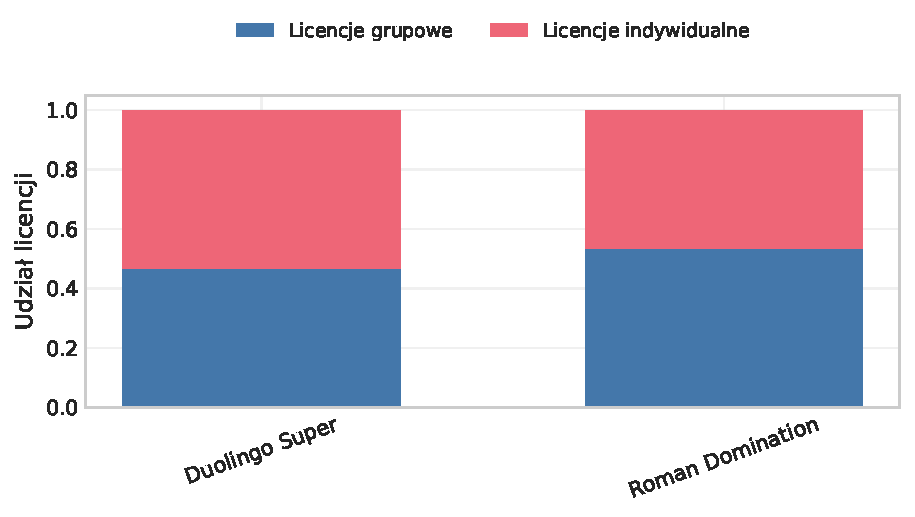
\includegraphics[width=0.6\linewidth]{assets/figures/benchmark/synthetic/license_mix_duo_vs_roman.pdf}
  \caption{Struktura wykorzystania licencji: porównanie konfiguracji licencyjnych Duolingo Super i dominowania rzymskiego.}
  \label{fig:duo-roman-license}
\end{figure}

\section{Wnioski}

Przeprowadzone eksperymenty wskazują, że schemat licencjonowania Duolingo Super zapewnia stabilne i powtarzalne wyniki. Spośród badanych metod najlepsze wyniki uzyskały algorytm mrówkowy oraz przeszukiwanie tabu. Algorytm mrówkowy osiąga najniższy koszt licencji na węzeł w grupie metaheurystyk, lecz wymaga dłuższego czasu działania. Przeszukiwanie tabu umożliwia uzyskanie porównywalnej jakości i jednocześnie zachowuje lepszy kompromis między kosztem a czasem obliczeń.

Solver ILP stanowi punkt odniesienia jakościowego, lecz jego zastosowanie ogranicza się do mniejszych instancji ze względu na częste przekroczenia limitu czasu. Proste heurystyki, takie jak algorytm zachłanny czy losowy, charakteryzują się bardzo krótkim czasem działania, ale rozwiązania mają istotnie wyższy koszt licencji na węzeł.

Wyniki potwierdzają również znaczenie struktury grafu. W przypadku grafów losowych i małoświatowych możliwe jest osiągnięcie rezultatów zbliżonych do solvera ILP, natomiast grafy bezskalowe okazały się trudniejsze i generowały wyższe koszty. Rysunek~\ref{fig:duo-real-size} pokazuje, że przeszukiwanie tabu utrzymuje niskie wartości kosztu licencji na węzeł nawet przy rosnącej liczbie wierzchołków, a czasy działania rosną umiarkowanie.

Porównanie ze schematem licencyjnym dominowania rzymskiego wskazuje, że schemat ten osiąga niższy koszt licencji na węzeł we wszystkich typach grafów. Wynika to z większego udziału licencji grupowych i niższego kosztu jednostkowego. W grafach małoświatowych schemat Duolingo Super charakteryzuje się krótszym czasem wykonania.
